% Gemini theme
% https://github.com/anishathalye/gemini

\documentclass[final]{beamer}

% ====================
% Packages
% ====================

\usepackage[T1]{fontenc}
\usepackage{lmodern}
\usepackage[orientation=portrait,size=a1,scale=1.0]{beamerposter}
\usetheme{gemini}
\usecolortheme{gemini}
\usepackage{graphicx}
\usepackage{booktabs}
\usepackage{tikz}
\usepackage{pgfplots}
\pgfplotsset{compat=1.14}
\usepackage{anyfontsize}

\usepackage{empheq}
\usepackage[many]{tcolorbox}

%%% Math settings
\usepackage{amssymb,amsmath,mathtools}

% bra-ket
\newcommand*\bra[1]{\langle{#1}|}
\newcommand*\ket[1]{|{#1}\rangle}

% rotated wigner function
\newcommand*{\wigner}{W(\omega z, \omega^{-1}z^{*};t)}

% ====================
% Lengths
% ====================

% If you have N columns, choose \sepwidth and \colwidth such that
% (N+1)*\sepwidth + N*\colwidth = \paperwidth
\newlength{\sepwidth}
\newlength{\colwidth}
\setlength{\sepwidth}{0.025\paperwidth}
\setlength{\colwidth}{0.4625\paperwidth}

\newcommand{\separatorcolumn}{\begin{column}{\sepwidth}\end{column}}

% ====================
% Title
% ====================

\title{Numerical and Analytical Analysis of Squeezed Vacuum States of Light by Means of Wigner Functions}

\author{Joonhyup Lee \inst{1} \and Yoonchan Jeong \inst{1}}

\institute[shortinst]{\inst{1} Department of Electrical and Computer Engineering,
Seoul National University}

% ====================
% Footer (optional)
% ====================

\footercontent{
  \hfill
  2023-1 Undergraduate Final Project
  \hfill
}
% (can be left out to remove footer)

% ====================
% Logo (optional)
% ====================

% use this to include logos on the left and/or right side of the header:
\logoright{
\includegraphics[height=7cm]{laser-symbol.jpg}}
\logoleft{
\includegraphics[height=7cm]{snu-symbol.png}}

% ====================
% Body
% ====================

\begin{document}

\begin{frame}[t]
  \begin{columns}[t]
    \separatorcolumn

    \begin{column}{\colwidth}
      \begin{block}{What is Squeezed Light?}
        Quantum mechanics tells us that the fundamental limitation of measurements is given by the uncertainty product $\Delta x\Delta p\ge\hbar/2$.
        Since all phenomena are inherently quantum, all generalized position and momentum variables cannot be measured with arbitrary precision.
        This is also true for the case of EM waves. Consider the TEM field given by:
        \[
          \vec{E}_{\mathbf{k},\lambda}(\vec{r},t)=\vec{e}_{\mathbf{k},\lambda}(p\cos{(\mathbf{k}\cdot\vec{r}-ckt)}+q\sin{(\mathbf{k}\cdot\vec{r}-ckt)})
        \]
        Here the coefficients $q$ and $p$ are the generalized position and momentum variables, and the uncertainty product satisfies
        \[
          \Delta p\Delta q \ge \frac{\hbar ck}{2\varepsilon_{0}L^{3}}
        \]
        If we rewrite $p\cos{\theta(t)}+q\sin{\theta(t)}=A\sin{(\theta(t)+\phi)}$, we can conclude that the phase and amplitude cannot be both measured with arbitrary precision.
        However, we may consider methods to suppress the uncertainty of $\Delta q$ at the cost of a bigger $\Delta p$.
        That is, we want to ``squeeze'' the uncertainty in one direction.
      \end{block}

      \begin{block}{Background: Quantization of the Maxwell Equations}
        We can phrase the Maxwell equations in terms of the vector potential $\vec{A}$ and scalar potential $\phi$ that satisfies
        $\vec{E}=-\nabla\phi-\partial_{t}\vec{A}$ and $\vec{B}=\nabla\times\vec{A}$ under the Coulomb gauge by:

        $(\nabla^{2}-\varepsilon_{0}\mu_{0}\partial_{t}^{2})\vec{A}=-\mu_{0}\vec{J}-\nabla(\partial_{t}\phi)$,
        $\nabla^{2}\phi=-\rho$

        It turns out that interpreting the vector potential for each mode and polarization as the annihilation operator $\hat{a}$ gives the energy of the electric field perfectly.
        \begin{empheq}[box=\tcbhighmath]{align*}
          \vec{A}=\vec{\alpha}e^{i(\mathbf{k}\cdot\vec{r}-\omega_{\mathbf{k}}t)}\Rightarrow\omega_{\mathbf{k}}^{2}=c^{2}k^{2},\vec{\alpha}\cdot\mathbf{k}=0\qquad
          \text{Harmonic Oscillator}\\
          \vec{A}_{\mathbf{k},\lambda}=\vec{e}_{\mathbf{k},\lambda}\Re\{\alpha_{\mathbf{k},\lambda}e^{i(\mathbf{k}\cdot\vec{r}-ckt)}\}(\mathbf{k}=2\pi(m,n,l)/L,\lambda=1,2)\quad\text{Per-mode}\\
          \hat{\alpha}_{\mathbf{k},\lambda}=(2\hbar/\varepsilon_{0}L^{3}ck)^{1/2}\hat{a}_{\mathbf{k},\lambda}\qquad
          \text{Annihilation operator for each mode}
        \end{empheq}
        That is, we only need to analyze the harmonic oscillator per mode/polarization.
      \end{block}

      \begin{block}{Background: Squeezing Operator and the Wigner Function}
        The time evolution of a density operator in quantum mechanics can be represented by a unitary operation.
        We say that the density operator is squeezed when it is related to the original density operator by a unitary operator $S(\alpha)$ defined as below:
        \[S(\alpha)\coloneq\exp(i\cdot\Im\{\alpha^{*} \hat{a}^{2}\})\]
        The evolved density operator $S(\alpha)\rho S(\alpha)^{\dag}$ is said to be ``squeezed'' because the ``probability distribution'' is squeezed by the unitary transformation.
        The ``quasiprobability distribution'' function, or the ``Wigner function'' is defined as:
        \begin{empheq}[box=\tcbhighmath]{align*}
          W(q,p)=\frac{1}{\pi\hbar}\int_{-\infty}^{\infty}\bra{q-y}\rho\ket{q+y}e^{2ipy/\hbar}dy\qquad
          \text{Wigner function}
        \end{empheq}
        The time evolution of the Wigner function is governed by the Von Neumann equation $i\hbar\partial_{t}\rho=[H,\rho]$ adapted to the Wigner function by the following correspondence:
        \begin{align*}
          a\rho         & \leftrightarrow \left(z+\frac{1}{2}\partial_{z^{*}}\right)W & z                & \leftrightarrow q+ip                                    \\
          a^{\dag}\rho  & \leftrightarrow \left(z^{*}-\frac{1}{2}\partial_{z}\right)W & z^{*}            & \leftrightarrow q-ip                                    \\
          \rho a        & \leftrightarrow \left(z-\frac{1}{2}\partial_{z^{*}}\right)W & \partial_{z}     & \leftrightarrow \frac{1}{2}(\partial_{q}-i\partial_{p}) \\
          \rho a^{\dag} & \leftrightarrow \left(z^{*}-\frac{1}{2}\partial_{z}\right)W & \partial_{z^{*}} & \leftrightarrow \frac{1}{2}(\partial_{q}+i\partial_{p})
        \end{align*}
      \end{block} 
      \begin{block}{Background: Parametric Amplification}
        \begin{columns}
          \begin{column}{0.3\colwidth}
            \begin{figure}
              \begin{tikzpicture}[>=stealth]
                % Define the coordinates
                \coordinate (O) at (0,3);
                \coordinate (O') at (0,1);
                \coordinate (P) at (3,3);
                \coordinate (P') at (3,1);
                \coordinate (C) at (5,2);
                \coordinate (Q) at (7,3);
                \coordinate (R) at (10,3);

                % Draw the incident wave
                \draw[ultra thick, blue, ->] (O) -- (P) node[midway, above]
                {$\omega_{s}=\omega$};
                \draw[ultra thick, blue, ->] (O') -- (P') node[midway, above] {$\omega_{p}=2\omega$};

                % Draw the second harmonic wave
                \draw[ultra thick, red, ->] (Q) -- (R) node[midway, above] {$\omega_{i}$};

                % Draw the crystal
                \draw[thick, dashed] (3,-2) rectangle (7,6);

                % Draw the labels
                \node[above] at (C) {$\chi^{(2)}$};
                \node[below] at (C) {Crystal};
                \node[below right, red] at (Q) {$=\omega_{p}-\omega_{s}$};
              \end{tikzpicture}
              \caption{Parametric amplification using a second-order nonlinear crystal.}
            \end{figure}
          \end{column}
          \begin{column}{0.7\colwidth}
            \\
            The Hamiltonian inside the cavity between the signal and pump photons can be expressed as:
            \begin{empheq}[box=\tcbhighmath]{align*}
              \hat{H}=&\hbar\omega (\hat{a}^{\dag}\hat{a}+\frac{1}{2})+\hbar\omega_{p}(\hat{a_{p}}^{\dag}\hat{a_{p}}+\frac{1}{2})+\\
              &\underbrace{\frac{i\hbar\chi^{(2)}}{2}(\hat{a}^{2}\hat{a_{p}}^{\dag}-(\hat{a}^{\dag})^{2}\hat{a_{p}})}_{\text{second-order interaction}}\\
              \Rightarrow&\hbar\omega\hat{a}^{\dag}\hat{a}+\hbar\chi^{(2)}\Im\{\underbrace{\alpha^{*} e^{i\omega_{p}t}}_{\text{approx. }\hat{a_{p}}^{\dag}}\hat{a}^{2}\}
            \end{empheq}
            Let $\rho=\exp(-i\omega ta^{\dag}a)\tilde{\rho}\exp(i\omega ta^{\dag}a)$, then
            \[\partial_{t}\tilde{\rho}=-\frac{\chi^{(2)}}{2}(\alpha^{*}[a^{2},\tilde{\rho}]-\alpha[(a^{\dag})^{2},\tilde{\rho}])\]
            which is exactly the squeezing operator.
            The squeezed vacuum state of light is generated when the signal photon is at the state $\ket{0}$.
          \end{column}
        \end{columns}
      \end{block}


    \end{column}

    \separatorcolumn

    \begin{column}{\colwidth}
      \begin{block}{Numerical Analysis using QuTiP}
        As a first step to understanding the squeezed vacuum states of light, numerical simulation using the Python library QuTiP is employed.
        QuTiP simulates quantum phenomena by solving the Lindblad master equation in finite dimensional Hilbert space spanned by the number states $\{\ket{n}\}_{n=0}^{N}$.
        The Lindblad master equation is given by
        \[\partial_{t}\rho=-\frac{i}{\hbar}\underbrace{[H_{sys},\rho]}_{\text{system}}+\underbrace{\frac{1}{2}\sum_{n}(2C_{n}\rho C_{n}^{\dag}-\rho C_{n}^{\dag}C_{n}-C_{n}^{\dag} C_{n}\rho)}_{\text{environment}}\]
        and this models the case when the system we are interested in interacts with the environment by operators $C_{n}$.
        To test out the effectiveness of this approach, we plug in $H_{sys}$ as is described above, and $C_{n}=\sqrt{\gamma}\hat{a}$, that is, when the cavity loses photons to the surrounding environment.
        Plotting the Wigner function at time $5$ gives a figure:
        \begin{columns}
          \begin{column}{0.5\textwidth}
            \begin{figure}
              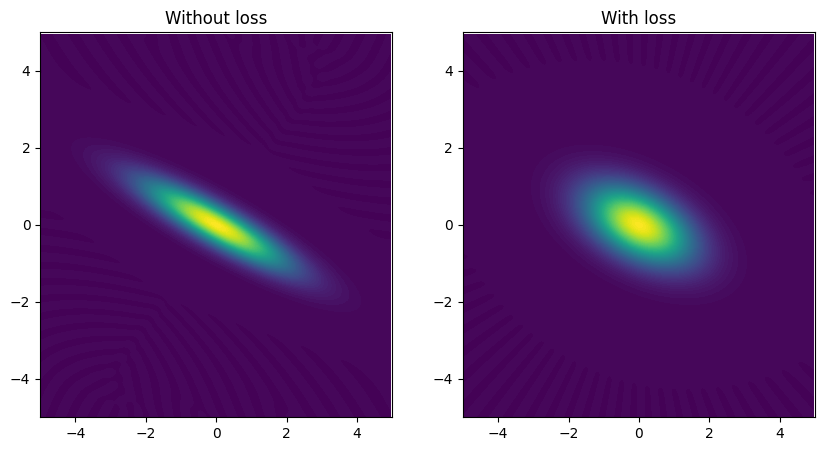
\includegraphics[width=0.5\textwidth]{squeezed_decay_0.5.png}
              \caption{Squeezing by a second-order interaction, compared with the case where the photons are lost to the environment by $\sqrt{\gamma}\hat{a}$. Here, $\alpha$ in $H_{sys}$ is chosen to be $0.2$, and $\gamma$ is chosen to be $0.5$.}
            \end{figure}
          \end{column}
          \begin{column}{0.5\textwidth}
            \begin{figure}
              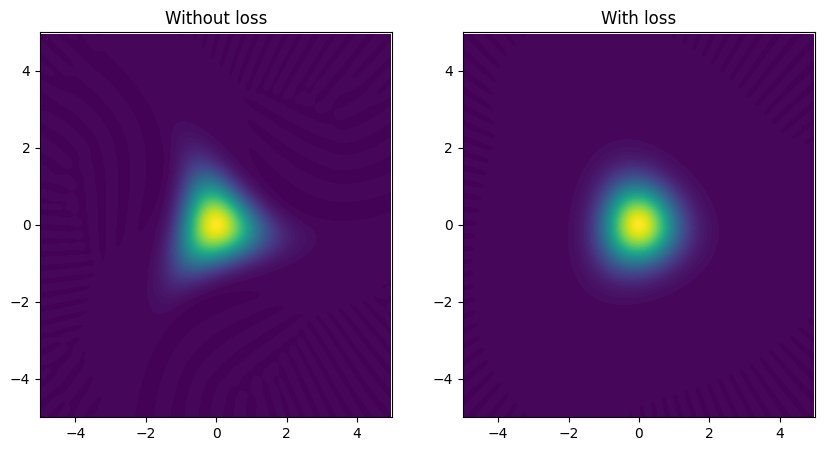
\includegraphics[width=0.5\textwidth]{third_decay_0.5.png}
              \caption{Squeezing by a third-order interaction, compared with the case where the photons are lost to the environment by $\sqrt{\gamma}\hat{a}$. Here, $\alpha$ in $H_{sys}$ is chosen to be $0.2$, and $\gamma$ is chosen to be $0.5$.}
            \end{figure}
          \end{column}
        \end{columns}
        As can be expected, the Wigner function is transformed into an ellipse, and the lossy distribution displays a level of squeezing much smaller than the non-lossy situation.

        Furthermore, to simulate the Wigner function that is not calculable by hand, the Wigner function of a squeezed state generated by a third-order interaction was also simulated in Figure 3.
        The $H_{sys}$ is given by $\hbar\omega\hat{a}^{\dag}\hat{a}+\hbar\chi^{(3)}\Im\{\underbrace{\alpha^{*} e^{i\omega_{p}t}}_{\text{approx. }\hat{a_{p}}^{\dag}}\hat{a}^{3}\}$ when $\omega_{p}=3\omega$, since the interaction is of third order.

        Here, we can see that the Wigner function evolves to something that looks like an equilateral triangle.
        The remaining sections serve to explain analytically why the Wigner functions evolve to what they are predicted in the above figures.
      \end{block}
      \begin{block}{Analytical Analysis: Second Order Squeezing is Linear in Phase Space}

        We show that for \textit{any} initial configuration, the Von Neumann equation dictates the Wigner function to be transformed by a squeezing operator.

        The Von Neumann equation turns into
        \[\partial_{t}W=-\frac{\chi^{(2)}}{2}(2\alpha z^{*}\partial_{z}W+2\alpha^{*}z\partial_{z^{*}}W)\]

        Now we want to evaluate how the Wigner function evolves in time given the distribution at time $0$.
        That is, we want to calculate the trajectory $(q(t), p(t))$ that satisfies $W(q(t),p(t);t)=W(q(0),p(0);0)$
        for all time $t$.

        Differentiating both sides by $t$, we get, by the chain rule,
        $z^{\prime}\partial_{z}W+z^{*\prime}\partial_{z^{*}}W+\partial_{t}W=0$
        if we view $W$ as a function of $z=q+ip$ and $z^{*}=q-ip$.

        By the time evolution equation, this equation can be summarized into
        $(z^{\prime}-\chi^{(2)}\alpha z^{*})\partial_{z}W+(z^{*\prime}-\chi^{(2)}\alpha^{*} z)\partial_{z^{*}}W=0$.

        Therefore, if the trajectory $z(t)=q(t)+ip(t)$ satisfies $\dfrac{dz}{dt}=\chi^{(2)}\alpha z^{*}$
        then for any initial condition we can determine the Wigner function at time $t$.
        This linear ode solves into:
        \[
          \begin{bmatrix}
            q \\
            p
          \end{bmatrix}
          =
          R_{\theta/2}
          \begin{bmatrix}
            e^{\chi^{(2)}rt} & 0                 \\
            0                & e^{-\chi^{(2)}rt}
          \end{bmatrix}
          R_{-\theta/2}
          \begin{bmatrix}
            q(0) \\
            p(0)
          \end{bmatrix}
        \]
        when $\alpha=re^{i\theta}$ and $R_{\theta/2}$ is the rotation matrix by $\theta/2$.

      \end{block}

      \begin{block}{Analytical Analysis: Third Order Squeezing Preserves Symmetry}

        We show that for an initial configuration that is symmetric to $R_{2\pi/3}$, the symmetry is preserved.

        The time evolution of the Wigner function is given by
        \[\partial_{t}W=-\frac{\chi^{(3)}}{2}\left(\alpha^{*}\left(3z^{2}\partial_{z^{*}}W+\frac{1}{4}\partial_{z^{*}}^{3}W\right)+\alpha\left(3(z^{*})^{2}\partial_{z}W+\frac{1}{4}\partial_{z}^{3}W\right)\right)\]

        We consider the rotated distribution $\tilde{W}(z,z^{*};t)\coloneq W(\omega z, \omega^{-1}z^{*};t)$ when $\omega=\exp(i2\pi/3)$ is the third root of unity.
        Note that
        \begin{align*}
          \partial_{t}\tilde{W}(z,z^{*};t)     & =\partial_{t}\wigner               \\
          \partial_{z}\tilde{W}(z,z^{*};t)     & =\omega\partial_{z}\wigner         \\
          \partial_{z}^{2}\tilde{W}(z,z^{*};t) & =\omega^{2}\partial_{z}^{2}\wigner \\
          \partial_{z}^{3}\tilde{W}(z,z^{*};t) & =\partial_{3}^{3}\wigner
        \end{align*}
        by the chain rule, so the above equation holds for $\tilde{W}$ as well.

        Then we have:
        \[\partial_{t}(W-\tilde{W})=-\frac{\chi^{(3)}}{2}\left(\alpha^{*}\left(3z^{2}\partial_{z^{*}}+\frac{1}{4}\partial_{z^{*}}^{3}\right)+\alpha\left(3(z^{*})^{2}\partial_{z}+\frac{1}{4}\partial_{z}^{3}\right)\right)(W-\tilde{W})\]
        If we have that for time $0$, $(W-\tilde{W})(q,p;0)=0$, then for the rest of the time, $W-\tilde{W}$ stays $0$.
        Since the vacuum initial state is a standard normal Gaussian and is therefore symmetric to rotations of any angle, we can explain why the distribution evolves to an equilateral triangle.
      \end{block}

      \begin{block}{References}
        \nocite{*}
        \footnotesize{\bibliographystyle{plain}\bibliography{poster}}
      \end{block}
    \end{column}

    \separatorcolumn
  \end{columns}
\end{frame}

\end{document}
